\subsection{Определение тока в ветви с сопротивлением $R_3$ методом
  эквивалентного источника напряжения}

По отношению к одной из ветвей линейную цепь с несколькими
источниками можно представить одним эквивалентным ИН $U_0$ с
последовательно соединённым сопротивлением $R_0$ (рис. \ref*{fig:equivalence_1}).

\begin{figure}[!h]
  \centering
  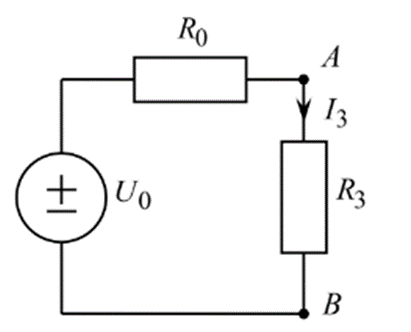
\includegraphics{equivalence_1.png}
  \caption{Эквивалентная схема}
  \label{fig:equivalence_1}
\end{figure}

Видно, что в данном случае
$$I_3 = \frac{U_0}{R_0 + R_3},$$
где $U_0$ — напряжение между выводами $A$ и $B$ ветви $3$ при обрыве
в данных точках, а $R_0$ — выходное сопротивление цепи со стороны
рассматриваемой ветви при исключении источников в схеме (рис. \ref*{fig:equivalence_2}).

\begin{figure}[!h]
  \centering
  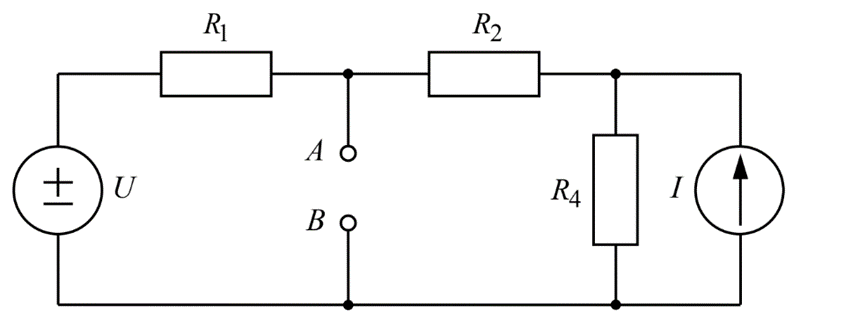
\includegraphics{equivalence_2.png}
  \caption{Схема с исключенным сопротивлением $R_3$}
  \label{fig:equivalence_2}
\end{figure}

\begin{equation}
  \begin{aligned}
     & \frac{1}{R_0}=\frac{1}{R_1}+\frac{1}{R_2+R_4}=\frac{1}{1,5 \text{кОм}} + \frac{1}{4,5 \text{кОм}} =\frac{4}{4,5 \text{кОм}}  \implies \\
     & \implies R_0=1,125 \text{кОм}
  \end{aligned}
\end{equation}

Теперь найдем $I_3$:

\begin{equation}
  I_3 = \frac{U_0}{R_0 + R_3} = \frac{2,20 \text{В}}{1,125 \text{кОм} + 3 \text{кОм}} = \frac{2,20 \text{В}}{4,125 \text{кОм}} = 0,533 \text{мА}
\end{equation}

Теоритический расчет показал, что ток в ветви с сопротивлением $R_3$
равен $0,533$ мА, что совпадает с результатами экспериментального
определения тока ($0,491$ мА) в ветви с сопротивлением $R_3$ с учётом погрешности.